\chapter{The ZMathLang Toolkit on an informal specification}

A specification describes a system as a list of requirements. The ZMathLang
toolkit assists users to analyse these requirements to check for loops in the
reasoning, identify inconsistencies, create evidence for a safety case and
ultimately proving the correctness of the specification. 

The ZMathLang toolkit does this in 6 steps.

\begin{enumerate}
    \item is the list of requirements written in plain English
    \item (ZCGa)- the user annotates the text which checks the grammar of the
    specification. E.g. if a term is defined more than once
    \item (ZDRa)- The user annotates the text and checks if there is any
    circular reasoning in the list of requirements. This step also generates a
    graph based on which requirements are dependent on each other.
    \item The list of requirements is put in an order based on the graph
    generated in the previous step.
    \item A skeleton is produced in a theorem prover languages for
    example Isabelle based on the list in the previous section.
    \item The skeleton is filled in and the entire specification is
    automatically translated into a theorem prover (such as Isabelle) ready to
    prove safety properties about the system.
\end{enumerate}

The proofs of the safety properties have to be done manually in the language of
the theorem prover.

\section{Step 0}

A specification is a list of requirements for autonomous vehicle

\noindent\fbox{%
    \parbox{\textwidth}{%
    \begin{enumerate}
    \item The vehicle shall stop at a red light
    \item The vehicle shall not kill any human being
    \item The vehicle shall not harm any human being
    \item The vehicle shall hand over control to the driver when requested 
    \item etc, etc
    \end{enumerate}
    }
}

\section{Step 1}
The user annotates the grammar of the requirements which help to identify
inconsistencies e.g. a term has been defined twice. 

For example System Engineer writes the following requirements:

\noindent\fbox{%
    \parbox{\textwidth}{%
    \begin{enumerate}
    \item The vehicle shall stop at a red light
    \item The vehicle shall not kill any human being
    \item The vehicle shall not harm any human being
    \item The vehicle shall hand over control to the driver when requested 
    \item A \term{driver}: \expression{shall\ be\ a\ human\ being\ over\ the\
    age\ of\ 18\ \\
    sitting\ inside\ the\ vehicle}
    \item etc, etc
    \end{enumerate}
    }
}

System engineer B writes the following set of requirements:

\noindent\fbox{%
    \parbox{\textwidth}{%
    \begin{enumerate}
    \item The driver shall be in sitting in a comfortable position in the vehicle.
    \item The \term{driver}:\expression{shall\ be\ a\ human\ being\ over\ the\
    age\ of\ 17\ \\
    sitting\ inside\ the\ vehicle}
    \item The driver shall be relaxed 
    \item etc, etc
    \end{enumerate}
    }
}

In this case the ZMathLang toolkit will flag up an error because requirement 5
from A conflicts with requirement 2 from B.

\section{Step 2}

The user annotates the requirements to check for loops. Loops may be difficult
to spot in a very large list of requirements particularly if the requirements have
been written by multiple people.

For example if we had the following list of requirements:

\noindent\fbox{%
    \parbox{\textwidth}{%
    \begin{enumerate}
    \item The Unmanned Air Vehicle takes command from the Wildcat Helicopter.
    \item The Unmanned Air Vehicle shall stay in it's allocated airspace.
    \item The Wildcat Helicopter takes command from the Chinook.
    \item The Wildcat Helicopter shall stay on base until told to deploy.
    \item The Chinook takes command from the Unmanned Air Vehicle.
    \end{enumerate}
    }
}


The user will then annotate these requirements

\dratheory{T5}{0.3}{
    
\draschema{CS1}{The Unmanned Air Vehicle takes command from the Wildcat Helicopter.}
\draschema{CS2}{The Unmanned Air Vehicle shall stay in it's allocated airspace.}
\draschema{CS3}{The Wildcat Helicopter takes command from the Chinook.}
\draschema{CS4}{The Wildcat Helicopter shall stay on base until told to deploy.}
\draschema{CS5}{The Chinook takes command from the Unmanned Air Vehicle.}

\uses{CS1}{CS2}
}

\begin{figure}[H]
    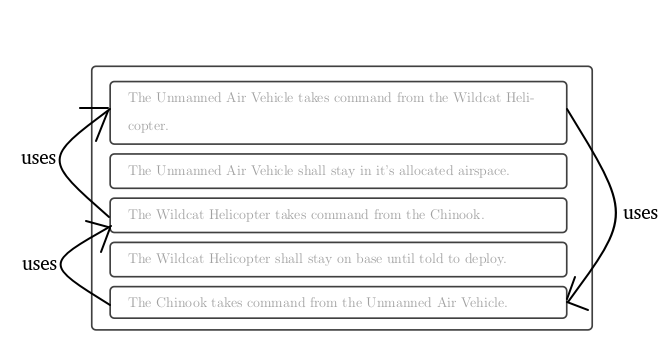
\includegraphics[width=12cm]{informal/zdra.png}
\end{figure}

The ZMathLang toolkit will identify the circular reasoning and tell the
user(requirements 1, 3 and 5). 
It will also produce the following graph to show that the 3 requirements are
dependent on each other and therefore show there is an error.

\begin{figure}[H]
    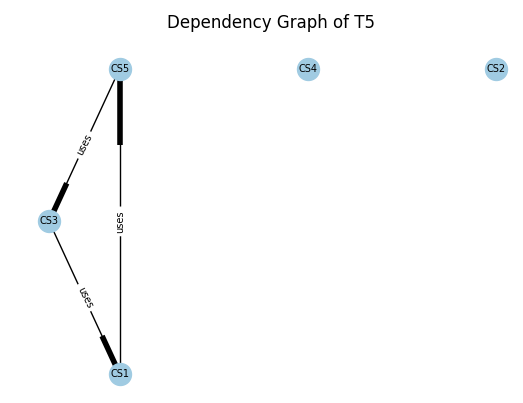
\includegraphics[width=12cm]{informal/dep.png}
\end{figure}

\section{Steps 3-6}

Sections 3-6 are specific to proving your specification is correct in a theorem
prover.
For example if your system has to stay in a particular state and the user
wishes to prove each function will not change the state of the system. Then the
toolkit will translate the specification (if written formally) into the theorem
prover isabelle and the user can prove that the state of the system doesnt
change.

\subsection{Step 3}
Step 3 lists the requirements in an order using the graph produced in Step 2.

For example if we had the following requirements

\noindent\fbox{%
    \parbox{\textwidth}{%
    \begin{enumerate}
    \item The vehicle shall stop at a red light
    \item The traffic lights shall display red green and amber
    \end{enumerate}
    }
}

In this example the first requirement is dependent on the second one. We can not
say \texttt{The vehicle shall stop at a red light} without defining when or what
is a red light. Therefore the ZMathLang toolkit will swap the order of these two
requirements.

\subsection{Step 4 and 5}

This translates your list of requirements (if written formally)  into the
theorem proving language Isabelle. An example of this is shown below.


\begin{figure}
    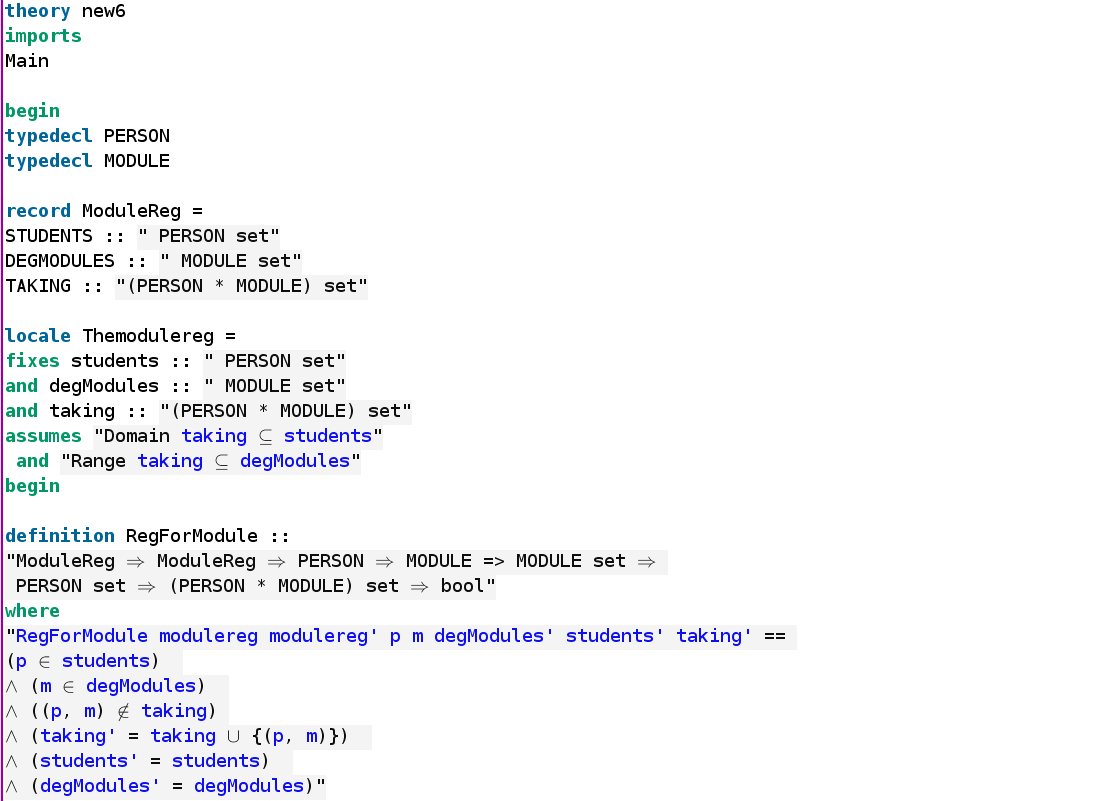
\includegraphics[width=\linewidth]{examples/modulereg/6imagea.png}
\end{figure}

\subsection{Step 6}

The finally step requires someone with expertise in the theorem proving language
Isabelle to prove properties about the specification.
An example of this is shown below.

\begin{figure}[H]
    \centering
    \begin{scriptsize}   
    \begin{BVerbatim}[commandchars=+\[\]] 
    lemma RegForModule_L1: "(\<exists>
    degModules:: MODULE set. \<exists> students ::
     PERSON set. \<exists> taking ::
    (PERSON * MODULE) set. \<exists> p :: PERSON. 
    \<exists> degModules':: MODULE
    set. \<exists> students' :: PERSON set. 
    \<exists> taking' :: (PERSON * MODULE)
    set. \<exists> m :: MODULE. ((p \<in> students) 
    \<and> (m \<in> degModules)
    \<and> ((p, m) \<notin> taking) \<and> 
    (taking' = taking \<union> {(p, m)})
    \<and> (students' = students) \<and> 
    (degModules' = degModules))
    \<longrightarrow> ((Domain taking 
    \<subseteq> students)  \<and> (Range taking
    \<subseteq> degModules) \<and> (Domain taking' 
    \<subseteq> students') \<and>
    (Range taking' \<subseteq> degModules')))"
    
    [+color[red]by (smt Domain_empty Domain_insert] 
    [+color[red]Range.intros
    Range_empty Range_insert]
    \end{BVerbatim}
    \end{scriptsize}
    \end{figure}